\documentclass[border=10pt]{standalone}
\usepackage{tikz}
\usetikzlibrary{matrix}

\providecommand{\lie}{\mathcal{L}}
\providecommand{\dext}{\textrm{d}}

\begin{document}
\tikzset{every loop/.style={min distance=10mm,looseness=10}}
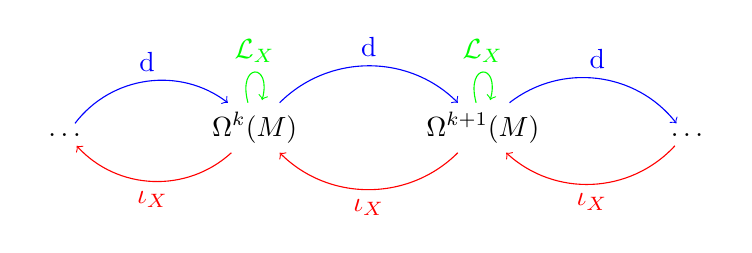
\begin{tikzpicture}
  \matrix (m) [matrix of math nodes,row sep=3em,column sep=4em,minimum width=2em]
  {
     \ldots & \Omega^k(M) & \Omega^{k+1}(M) & \ldots \\
     };
  \path[->]
    (m-1-1) edge[bend left=45,draw=blue] node [above,text=blue] {$\dext$} (m-1-2)
    (m-1-2) edge[bend left=45,draw=blue] node [above,text=blue] {$\dext$} (m-1-3)
    (m-1-3) edge[bend left=45,draw=blue] node [above,text=blue] {$\dext$} (m-1-4)
    (m-1-2) edge[bend left=45,draw=red] node [below,text=red] {$\iota_X$} (m-1-1)
    (m-1-3) edge[bend left=45,draw=red] node [below,text=red] {$\iota_X$} (m-1-2)
    (m-1-4) edge[bend left=45,draw=red] node [below,text=red] {$\iota_X$} (m-1-3)
    (m-1-2) edge [loop above,draw=green] node [above,text=green] {$\lie_X$} (m-1-2)
    (m-1-3) edge [loop above,draw=green] node [above,text=green] {$\lie_X$} (m-1-3)
	;
\end{tikzpicture}
\end{document}
